\section*{拟阵和复形}\addcontentsline{toc}{section}{拟阵和复形}
\sect{1\quad 引言}
\sect{2\quad 可壳复形}
先回顾基本定义。\textbf{单纯复形}（简称复形）$\Delta$ 是有限集 $V$ 的一个子集族，满足：(i) 若 $F\in\Delta$ 且 $G\subseteq F$，则 $G\in\Delta$；(ii) 对每个 $v\in V$，$\{v\}\in\Delta$。以下假定复形非空，因而 $\varnothing\in\Delta$。$V$ 的元素称为顶点，$\Delta$ 的元素称为单形或面。不真包含于其他面的面称为\textbf{刻面}。面的维数比其基数少一，复形的维数为面的最大维数，即
\[\dim F=|F|-1,\qquad\dim\Delta=\max\{\dim F:F\in\Delta\}.\]
若所有刻面等势，称复形为\textbf{纯}的。因此纯 $(r-1)$ 维复形的每个刻面都有 $r$ 个顶点；若刻面为 $F_1,\ldots,F_t$，则
\[\Delta=\bigcup_{i=1}^t2^{F_i},\qquad |F_i|=r.\]
这里 $2^{F_i}$ 包含 $F_i$ 的全部子面。纯性只要求刻面等维，并不限制它们如何相交；底层顶点集 $V$ 本身也未必是面。

令 $f_k$ 为基数为 $k$ 的面的个数，并令 $r=\dim\Delta+1$。于是 $f_0=1$、$f_1=|V|$，当 $k>r$ 时 $f_k=0$；边和三角形分别计入 $f_2$ 和 $f_3$。定义\textbf{面枚举多项式}为
\[f_\Delta(\lambda)=\lambda^r+f_1\lambda^{r-1}+\cdots+f_r=\sum_{i=0}^rf_i\lambda^{r-i}.\tag{3}\label{eq:complex-face}\]
定义 $\Delta$ 的\textbf{约化欧拉示性数}为
\[\chi(\Delta)=-1+f_1-f_2+\cdots=(-1)^{r-1}f_\Delta(-1).\]
若每个刻面都含同一顶点 $v$，称 $\Delta$ 为以 $v$ 为锥顶的\textbf{锥}。任一不含 $v$ 的面 $G$ 都包含于某个刻面 $F$，而 $v\in F$，故 $G\cup\{v\}\subseteq F$ 仍是面。因此可将面按 $G\longleftrightarrow G\cup\{v\}$ 一一配对，其中也包括空面与 $\{v\}$。每对面的基数相差一，贡献相消，故
\[\chi(\Delta)=0\qquad\text{若 }\Delta\text{ 是锥。}\tag{4}\]

\st{例35} 设 $\Delta$ 是图4中的二维单纯复形，其刻面为 $A=\{a,b,c\}$、$B=\{a,b,d\}$、$C=\{a,c,d\}$、$D=\{b,d,e\}$、$E=\{c,d,e\}$、$F=\{b,c,d\}$。其面数为 $f_0=1,f_1=5,f_2=9,f_3=6$，所以 $\chi(\Delta)=-1+5-9+6=1$。
\begin{center}
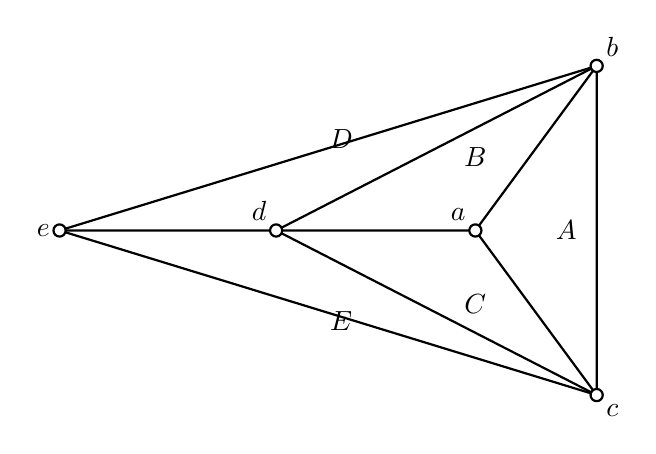
\begin{tikzpicture}[scale=1.1,line join=round]
\coordinate (e) at (0,0);\coordinate (d) at (2.5,0);\coordinate (a) at (4.8,0);\coordinate (b) at (6.2,1.9);\coordinate (c) at (6.2,-1.9);
\draw[thick] (e)--(b)--(c)--cycle;
\draw[thick] (e)--(d)--(a)--(b) (d)--(b) (d)--(c) (a)--(c);
\foreach \v/\pos in {e/left,d/above left,a/above left,b/above right,c/below right}{\filldraw[fill=white,thick] (\v) circle (2pt);\node[\pos] at (\v) {$\v$};}
\node at (5.85,0) {$A$};\node at (4.8,.85) {$B$};\node at (4.8,-.85) {$C$};\node at (3.25,1.05) {$D$};\node at (3.25,-1.05) {$E$};
\end{tikzpicture}\par\small 图4
\end{center}
图中画出各顶点和边，字母标出相应三角形；刻面 $F=\{b,c,d\}$ 与其他三角形在平面投影中重叠，未另标出。

设 $\Delta$ 为纯单纯复形。它的一个\textbf{壳序}是刻面的线性次序，使每个刻面（除第一个外）与此前刻面生成的复形的交，是其若干极大真面的非空并。这里，$F$ 的真面是严格包含于 $F$ 的面，其极大真面恰是删去一个顶点所得的面。因此，新刻面沿若干完整的余维一面贴入。换言之，刻面的线性次序 $F_1,\ldots,F_t$ 是壳序，当且仅当
\[\begin{gathered}
\text{对每对 }F_i,F_j\ (1\le i<j\le t),\text{存在 }F_k\ (1\le k<j)\text{ 及 }x\in F_j,\\
F_i\cap F_j\subseteq F_k\cap F_j=F_j\setminus\{x\}.
\end{gathered}\tag{5}\label{eq:shell-condition}\]
等号表示新刻面的一个完整余维一面已经出现；包含关系要求与任一旧刻面的交都落在这样的面中。这里 $k$ 不必等于 $i$：某个交即使维数较低，也可以由另一个旧刻面提供的余维一面覆盖，但不能成为粘合部分中孤立的低维部分。

纯复形若有壳序，称为\textbf{可壳}的。每个零维复形都可壳；一维复形（简单图）可壳当且仅当连通。壳序的直观含义是：逐次加入刻面来构造纯 $d$ 维复形，每次把新刻面很好地贴到已构造部分上，使交在拓扑上是 $(d-1)$ 维闭球或 $(d-1)$ 维球面。闭球与球面分别指
\[B^m=\{x\in\R^m:\|x\|\le1\},\qquad S^m=\{x\in\R^{m+1}:\|x\|=1\};\]
这里的“是”指同胚。粘合部分若为新单形边界的非空且非全部的余维一面之并，就同胚于 $B^{d-1}$；若为整个边界，就同胚于 $S^{d-1}$。

例如，取顶点集 $V=\{a,b,c,d\}$，令三个刻面依次为 $F_1=\{a,b,d\}$、$F_2=\{a,c,d\}$、$F_3=\{a,b,c\}$，并取它们的全部子面组成复形。这里 $V$ 本身不是面。加入 $F_2$ 时沿边 $ad$ 粘合；加入 $F_3$ 时同时沿边 $ab$ 和 $ac$ 粘合，两条边组成的“V”形同胚于闭线段 $B^1$。若再加入三角形 $bcd$，则沿其全部三条边粘合，交同胚于圆周 $S^1$；所得复形是四面体的边界，仍不包含四面体本身。

图4中，先将 $A,B,C$ 任意排列，再将 $D,E,F$ 任意排列，便得到壳序；但以 $A,B,E,\ldots$ 或 $D,E,C,A,\ldots$ 开始的次序不是壳序。

以下固定记号：$\Delta$ 是 $(r-1)$ 维可壳复形，$F_1,\ldots,F_t$ 按壳序排列。令
\[\Delta_i=\{G\in\Delta:G\subseteq F_k\text{ 对某个 }k\le i\},\qquad\Delta_0=\varnothing,\]
即前 $i$ 个刻面生成的子复形。对 $i=1,\ldots,t$，令
\[\mathcal R(F_i)=\{x\in F_i:F_i\setminus\{x\}\in\Delta_{i-1}\},\]
称为壳序诱导的 $F_i$ 的\textbf{限制面}。其中的顶点恰是那些删去后使剩余面已经出现的顶点。于是 $\mathcal R(F_i)=\varnothing$ 当且仅当 $i=1$；$\mathcal R(F_i)=F_i$ 当且仅当其所有真子集都属于 $\Delta_{i-1}$。

把 $\Delta$ 按面的包含关系排序，可在其中考虑\textbf{布尔区间}
\[[G_1,G_2]=\{G:G_1\subseteq G\subseteq G_2\}.\]

\st{命题36} 区间 $[\mathcal R(F_i),F_i]$（$i=1,\ldots,t$）划分可壳复形 $\Delta$。
这里的划分是对面族 $\Delta$ 的集合意义下的划分：每个面恰好属于一个区间。事实上，第 $i$ 个区间正是加入 $F_i$ 时首次出现的全部面。
\pr $F_1,\ldots,F_i$ 是 $\Delta_i$ 的壳序，故归纳地只需证明：(i) $\Delta_{t-1}\cup[\mathcal R(F_t),F_t]=\Delta$；(ii) $\Delta_{t-1}\cap[\mathcal R(F_t),F_t]=\varnothing$。若 $G\in\Delta\setminus\Delta_{t-1}$，则 $G\subseteq F_t$。若某个 $x\in\mathcal R(F_t)$ 不属于 $G$，则 $G\subseteq F_t\setminus\{x\}\in\Delta_{t-1}$，矛盾。因此 $\mathcal R(F_t)\subseteq G$，得到(i)。

(ii)等价于 $\mathcal R(F_t)\notin\Delta_{t-1}$：因为区间中的每个面都包含 $\mathcal R(F_t)$，而旧复形对子集封闭。若不然，则对某个 $i<t$，$\mathcal R(F_t)\subseteq F_i\cap F_t$。由式\eqref{eq:shell-condition}，存在 $k<t$ 及 $x\in F_t$，使
\[\mathcal R(F_t)\subseteq F_i\cap F_t\subseteq F_k\cap F_t=F_t\setminus\{x\}.\]
然而 $F_t\setminus\{x\}\subseteq F_k\in\Delta_{t-1}$ 蕴含 $x\in\mathcal R(F_t)$，与 $\mathcal R(F_t)\subseteq F_t\setminus\{x\}$ 矛盾。\qed

这表明：在壳化过程中把刻面 $F_i$ 及其子面加入 $\Delta_{i-1}$ 时，$\mathcal R(F_i)$ 是 $F_i$ 中唯一极小的“新”面，即属于 $\Delta_i\setminus\Delta_{i-1}$ 的极小面。本步新增的恰是 $F_i$ 中包含整个 $\mathcal R(F_i)$ 的那些子面。定义可壳复形的\textbf{壳多项式}为
\[h_\Delta(x)=\sum_{i=1}^t x^{|F_i\setminus\mathcal R(F_i)|}.\tag{6}\label{eq:shell-polynomial}\]
限制面依赖于所选壳序，同一刻面在不同壳序中的限制面及其大小都可能改变；但下述命题说明，壳多项式与壳序无关。

\st{命题37} 若 $\Delta$ 可壳，则 $h_\Delta(1+\lambda)=f_\Delta(\lambda)$。因此壳多项式与壳序选择无关。
\pr 由命题36，第 $i$ 步新增的面组成区间 $[\mathcal R(F_i),F_i]$。记 $m_i=|F_i\setminus\mathcal R(F_i)|$。这些面必须保留限制面中的全部顶点，其余 $m_i$ 个顶点可自由选择。从 $F_i$ 中删去其中 $j$ 个顶点，就得到一个大小为 $r-j$ 的新面，在面枚举多项式中贡献 $\lambda^j$。因此，第 $i$ 步的贡献为
\[\sum_{j=0}^{m_i}\binom{m_i}{j}\lambda^j=(1+\lambda)^{m_i}.\]
各步新增的面无交地覆盖 $\Delta$，求和得到
\[f_\Delta(\lambda)=\sum_{i=1}^t(1+\lambda)^{m_i}=h_\Delta(1+\lambda).\]
于是 $h_\Delta(x)=f_\Delta(x-1)$，右侧只由复形的面数决定，故与壳序选择无关。\qed

所以 $h_\Delta(1)$ 等于刻面数，$h_\Delta(2)$ 等于总面数。更重要的是
\[h_\Delta(0)=f_\Delta(-1)=(-1)^{r-1}\chi(\Delta).\]
另一方面，由定义它等于满足 $\mathcal R(F)=F$ 的刻面数。因此：
\st{推论38} $(-1)^{r-1}\chi(\Delta)$ 等于满足 $\mathcal R(F)=F$ 的刻面 $F$ 的个数。\qed

\sect{3\quad 拟阵复形}
\sect{4\quad 断路复形}
\sect{5\quad 拟阵不等式的应用}
